
%% bare_conf.tex
%% V1.4b
%% 2015/08/26
%% by Michael Shell
%% See:
%% http://www.michaelshell.org/
%% for current contact information.
%%
%% This is a skeleton file demonstrating the use of IEEEtran.cls
%% (requires IEEEtran.cls version 1.8b or later) with an IEEE
%% conference paper.
%%
%% Support sites:
%% http://www.michaelshell.org/tex/ieeetran/
%% http://www.ctan.org/pkg/ieeetran
%% and
%% http://www.ieee.org/

%%*************************************************************************
%% Legal Notice:
%% This code is offered as-is without any warranty either expressed or
%% implied; without even the implied warranty of MERCHANTABILITY or
%% FITNESS FOR A PARTICULAR PURPOSE! 
%% User assumes all risk.
%% In no event shall the IEEE or any contributor to this code be liable for
%% any damages or losses, including, but not limited to, incidental,
%% consequential, or any other damages, resulting from the use or misuse
%% of any information contained here.
%%
%% All comments are the opinions of their respective authors and are not
%% necessarily endorsed by the IEEE.
%%
%% This work is distributed under the LaTeX Project Public License (LPPL)
%% ( http://www.latex-project.org/ ) version 1.3, and may be freely used,
%% distributed and modified. A copy of the LPPL, version 1.3, is included
%% in the base LaTeX documentation of all distributions of LaTeX released
%% 2003/12/01 or later.
%% Retain all contribution notices and credits.
%% ** Modified files should be clearly indicated as such, including  **
%% ** renaming them and changing author support contact information. **
%%*************************************************************************


% *** Authors should verify (and, if needed, correct) their LaTeX system  ***
% *** with the testflow diagnostic prior to trusting their LaTeX platform ***
% *** with production work. The IEEE's font choices and paper sizes can   ***
% *** trigger bugs that do not appear when using other class files.       ***                          ***
% The testflow support page is at:
% http://www.michaelshell.org/tex/testflow/



\documentclass[conference]{IEEEtran}
% Some Computer Society conferences also require the compsoc mode option,
% but others use the standard conference format.
%
% If IEEEtran.cls has not been installed into the LaTeX system files,
% manually specify the path to it like:
% \documentclass[conference]{../sty/IEEEtran}


% Using this only for editing/TODO/commenting purposes.
% TODO: Remove this in the final version.
\usepackage{color}
%Cherry added this to have unordered lists in the paper.
\usepackage{enumitem}
%Cherry added this to have upper-case Greek letters.
\usepackage{upgreek}
%Cherry added this to be able to write lemmas and proofs
\usepackage{amsthm}
\theoremstyle{plain}% default
\newtheorem{theorem}{Theorem}[section]
\newtheorem{lemma}[theorem]{Lemma}
\newtheorem{claim}[theorem]{Claim}
%Cherry added this to use \norm
\usepackage{commath}
%Cherry added this to add the Z integer symbol.
\usepackage{ dsfont }

% Some very useful LaTeX packages include:
% (uncomment the ones you want to load)


% *** MISC UTILITY PACKAGES ***
%
%\usepackage{ifpdf}
% Heiko Oberdiek's ifpdf.sty is very useful if you need conditional
% compilation based on whether the output is pdf or dvi.
% usage:
% \ifpdf
%   % pdf code
% \else
%   % dvi code
% \fi
% The latest version of ifpdf.sty can be obtained from:
% http://www.ctan.org/pkg/ifpdf
% Also, note that IEEEtran.cls V1.7 and later provides a builtin
% \ifCLASSINFOpdf conditional that works the same way.
% When switching from latex to pdflatex and vice-versa, the compiler may
% have to be run twice to clear warning/error messages.






% *** CITATION PACKAGES ***
%
\usepackage{cite}
% cite.sty was written by Donald Arseneau
% V1.6 and later of IEEEtran pre-defines the format of the cite.sty package
% \cite{} output to follow that of the IEEE. Loading the cite package will
% result in citation numbers being automatically sorted and properly
% "compressed/ranged". e.g., [1], [9], [2], [7], [5], [6] without using
% cite.sty will become [1], [2], [5]--[7], [9] using cite.sty. cite.sty's
% \cite will automatically add leading space, if needed. Use cite.sty's
% noadjust option (cite.sty V3.8 and later) if you want to turn this off
% such as if a citation ever needs to be enclosed in parenthesis.
% cite.sty is already installed on most LaTeX systems. Be sure and use
% version 5.0 (2009-03-20) and later if using hyperref.sty.
% The latest version can be obtained at:
% http://www.ctan.org/pkg/cite
% The documentation is contained in the cite.sty file itself.






% *** GRAPHICS RELATED PACKAGES ***
%
\ifCLASSINFOpdf
   \usepackage[pdftex]{graphicx}
  % declare the path(s) where your graphic files are
   \graphicspath{{images/}}
  % and their extensions so you won't have to specify these with
  % every instance of \includegraphics
  \DeclareGraphicsExtensions{.pdf,.jpeg,.png,.jpg}
\else
  % or other class option (dvipsone, dvipdf, if not using dvips). graphicx
  % will default to the driver specified in the system graphics.cfg if no
  % driver is specified.
  \usepackage[dvips]{graphicx}
  % declare the path(s) where your graphic files are
  \graphicspath{{images/}}
  % and their extensions so you won't have to specify these with
  % every instance of \includegraphics
  % \DeclareGraphicsExtensions{.eps}
\fi
% graphicx was written by David Carlisle and Sebastian Rahtz. It is
% required if you want graphics, photos, etc. graphicx.sty is already
% installed on most LaTeX systems. The latest version and documentation
% can be obtained at: 
% http://www.ctan.org/pkg/graphicx
% Another good source of documentation is "Using Imported Graphics in
% LaTeX2e" by Keith Reckdahl which can be found at:
% http://www.ctan.org/pkg/epslatex
%
% latex, and pdflatex in dvi mode, support graphics in encapsulated
% postscript (.eps) format. pdflatex in pdf mode supports graphics
% in .pdf, .jpeg, .png and .mps (metapost) formats. Users should ensure
% that all non-photo figures use a vector format (.eps, .pdf, .mps) and
% not a bitmapped formats (.jpeg, .png). The IEEE frowns on bitmapped formats
% which can result in "jaggedy"/blurry rendering of lines and letters as
% well as large increases in file sizes.
%
% You can find documentation about the pdfTeX application at:
% http://www.tug.org/applications/pdftex





% *** MATH PACKAGES ***
%
\usepackage{amsmath}
% A popular package from the American Mathematical Society that provides
% many useful and powerful commands for dealing with mathematics.
%
% Note that the amsmath package sets \interdisplaylinepenalty to 10000
% thus preventing page breaks from occurring within multiline equations. Use:
%\interdisplaylinepenalty=2500
% after loading amsmath to restore such page breaks as IEEEtran.cls normally
% does. amsmath.sty is already installed on most LaTeX systems. The latest
% version and documentation can be obtained at:
% http://www.ctan.org/pkg/amsmath





% *** SPECIALIZED LIST PACKAGES ***
%
\usepackage{algorithmic}
\usepackage{algorithm}
% algorithmic.sty was written by Peter Williams and Rogerio Brito.
% This package provides an algorithmic environment for describing algorithms.
% You can use the algorithmic environment in-text or within a figure
% environment to provide for a floating algorithm. Do NOT use the algorithm
% floating environment provided by algorithm.sty (by the same authors) or
% algorithm2e.sty (by Christophe Fiorio) as the IEEE does not use dedicated
% algorithm float types and packages that provide these will not provide
% correct IEEE style captions. The latest version and documentation of
% algorithmic.sty can be obtained at:
% http://www.ctan.org/pkg/algorithms
% Also of interest may be the (relatively newer and more customizable)
% algorithmicx.sty package by Szasz Janos:
% http://www.ctan.org/pkg/algorithmicx

%Cherry added this to add break command in algorithmic
\newcommand{\algorithmicbreak}{\textbf{break}}
\newcommand{\BREAK}{\STATE \algorithmicbreak}

% *** ALIGNMENT PACKAGES ***
%
%\usepackage{array}
% Frank Mittelbach's and David Carlisle's array.sty patches and improves
% the standard LaTeX2e array and tabular environments to provide better
% appearance and additional user controls. As the default LaTeX2e table
% generation code is lacking to the point of almost being broken with
% respect to the quality of the end results, all users are strongly
% advised to use an enhanced (at the very least that provided by array.sty)
% set of table tools. array.sty is already installed on most systems. The
% latest version and documentation can be obtained at:
% http://www.ctan.org/pkg/array


% IEEEtran contains the IEEEeqnarray family of commands that can be used to
% generate multiline equations as well as matrices, tables, etc., of high
% quality.




% *** SUBFIGURE PACKAGES ***
%\ifCLASSOPTIONcompsoc
%  \usepackage[caption=false,font=normalsize,labelfont=sf,textfont=sf]{subfig}
%\else
%  \usepackage[caption=false,font=footnotesize]{subfig}
%\fi
% subfig.sty, written by Steven Douglas Cochran, is the modern replacement
% for subfigure.sty, the latter of which is no longer maintained and is
% incompatible with some LaTeX packages including fixltx2e. However,
% subfig.sty requires and automatically loads Axel Sommerfeldt's caption.sty
% which will override IEEEtran.cls' handling of captions and this will result
% in non-IEEE style figure/table captions. To prevent this problem, be sure
% and invoke subfig.sty's "caption=false" package option (available since
% subfig.sty version 1.3, 2005/06/28) as this is will preserve IEEEtran.cls
% handling of captions.
% Note that the Computer Society format requires a larger sans serif font
% than the serif footnote size font used in traditional IEEE formatting
% and thus the need to invoke different subfig.sty package options depending
% on whether compsoc mode has been enabled.
%
% The latest version and documentation of subfig.sty can be obtained at:
% http://www.ctan.org/pkg/subfig




% *** FLOAT PACKAGES ***
%
%\usepackage{fixltx2e}
% fixltx2e, the successor to the earlier fix2col.sty, was written by
% Frank Mittelbach and David Carlisle. This package corrects a few problems
% in the LaTeX2e kernel, the most notable of which is that in current
% LaTeX2e releases, the ordering of single and double column floats is not
% guaranteed to be preserved. Thus, an unpatched LaTeX2e can allow a
% single column figure to be placed prior to an earlier double column
% figure.
% Be aware that LaTeX2e kernels dated 2015 and later have fixltx2e.sty's
% corrections already built into the system in which case a warning will
% be issued if an attempt is made to load fixltx2e.sty as it is no longer
% needed.
% The latest version and documentation can be found at:
% http://www.ctan.org/pkg/fixltx2e


%\usepackage{stfloats}
% stfloats.sty was written by Sigitas Tolusis. This package gives LaTeX2e
% the ability to do double column floats at the bottom of the page as well
% as the top. (e.g., "\begin{figure*}[!b]" is not normally possible in
% LaTeX2e). It also provides a command:
%\fnbelowfloat
% to enable the placement of footnotes below bottom floats (the standard
% LaTeX2e kernel puts them above bottom floats). This is an invasive package
% which rewrites many portions of the LaTeX2e float routines. It may not work
% with other packages that modify the LaTeX2e float routines. The latest
% version and documentation can be obtained at:
% http://www.ctan.org/pkg/stfloats
% Do not use the stfloats baselinefloat ability as the IEEE does not allow
% \baselineskip to stretch. Authors submitting work to the IEEE should note
% that the IEEE rarely uses double column equations and that authors should try
% to avoid such use. Do not be tempted to use the cuted.sty or midfloat.sty
% packages (also by Sigitas Tolusis) as the IEEE does not format its papers in
% such ways.
% Do not attempt to use stfloats with fixltx2e as they are incompatible.
% Instead, use Morten Hogholm'a dblfloatfix which combines the features
% of both fixltx2e and stfloats:
%
% \usepackage{dblfloatfix}
% The latest version can be found at:
% http://www.ctan.org/pkg/dblfloatfix




% *** PDF, URL AND HYPERLINK PACKAGES ***
%
%\usepackage{url}
% url.sty was written by Donald Arseneau. It provides better support for
% handling and breaking URLs. url.sty is already installed on most LaTeX
% systems. The latest version and documentation can be obtained at:
% http://www.ctan.org/pkg/url
% Basically, \url{my_url_here}.




% *** Do not adjust lengths that control margins, column widths, etc. ***
% *** Do not use packages that alter fonts (such as pslatex).         ***
% There should be no need to do such things with IEEEtran.cls V1.6 and later.
% (Unless specifically asked to do so by the journal or conference you plan
% to submit to, of course. )

\begin{document}
%
% paper title
% Titles are generally capitalized except for words such as a, an, and, as,
% at, but, by, for, in, nor, of, on, or, the, to and up, which are usually
% not capitalized unless they are the first or last word of the title.
% Linebreaks \\ can be used within to get better formatting as desired.
% Do not put math or special symbols in the title.
\title{Minimizing Turns and Altitude Changes 
\\ in a 3D Sweeping Coverage Problem for UAVs}

% author names and affiliations
% use a multiple column layout for up to three different
% affiliations
\author{\IEEEauthorblockN{Yingzi Zhang}
\IEEEauthorblockA{Dept. of Mechanical and\\Mechatronics Engineering\\
University of Waterloo\\
Waterloo, ON N2L 3G1\\
Email: y689zhan@uwaterloo.ca}
\and
\IEEEauthorblockN{Stephen L. Smith}
\IEEEauthorblockA{Dept. of Electrical and\\Computer Engineering\\
University of Waterloo\\
Waterloo, ON N2L 3G1\\
Email: stephen.smith@uwaterloo.ca}}

% conference papers do not typically use \thanks and this command
% is locked out in conference mode. If really needed, such as for
% the acknowledgment of grants, issue a \IEEEoverridecommandlockouts
% after \documentclass

% for over three affiliations, or if they all won't fit within the width
% of the page, use this alternative format:
% 
%\author{\IEEEauthorblockN{Michael Shell\IEEEauthorrefmark{1},
%Homer Simpson\IEEEauthorrefmark{2},
%James Kirk\IEEEauthorrefmark{3}, 
%Montgomery Scott\IEEEauthorrefmark{3} and
%Eldon Tyrell\IEEEauthorrefmark{4}}
%\IEEEauthorblockA{\IEEEauthorrefmark{1}School of Electrical and Computer Engineering\\
%Georgia Institute of Technology,
%Atlanta, Georgia 30332--0250\\ Email: see http://www.michaelshell.org/contact.html}
%\IEEEauthorblockA{\IEEEauthorrefmark{2}Twentieth Century Fox, Springfield, USA\\
%Email: homer@thesimpsons.com}
%\IEEEauthorblockA{\IEEEauthorrefmark{3}Starfleet Academy, San Francisco, California 96678-2391\\
%Telephone: (800) 555--1212, Fax: (888) 555--1212}
%\IEEEauthorblockA{\IEEEauthorrefmark{4}Tyrell Inc., 123 Replicant Street, Los Angeles, California 90210--4321}}

% use for special paper notices
%\IEEEspecialpapernotice{(Invited Paper)}

% make the title area
\maketitle{}

% As a general rule, do not put math, special symbols or citations
% in the abstract
% TODO: Rewrite this abstract to make it better.
\begin{abstract}
The sweeping coverage problem has been looked at extensively in literature, particularly in scenarios where UAVs must capture photographs of a large 2D area. We attempt to look at this problem where the UAV can move in 3D instead of being conventionally restricted on a plane. It is important for the UAV to be able to move in 3D when the area to be covered does not have a uniformly-defined image-resolution requirement, but instead, has several sub-areas that need to be captured in higher or lower resolutions. In this paper, we attempt to create an algorithm that allows the UAV to autonomously take images of the coverage area at the correct minimum-required resolutions. While there are some existing algorithms that can do this that minimize the total travel distance of the UAV, there does not seem to be one that minimizes the number of turns the UAV conducts, despite the fact that monitoring applications can benefit from minimal UAV turns in terms of image quality and in time. There is also benefit in minimizing the total number of altitude changes the UAV makes as well in order to minimize image distortion. Thus, we attempt to create a 3D path planning algorithm for the UAV to traverse such that we minimize both the number of turns and the number of total altitude changes. This is done using: a clustering algorithm that minimizes the number of altitude changes by grouping regions of similar image-resolution values under one uniform image-resolution, and a CGTSP tour of the clusters such that rotations are minimized. In addition, we provide a focal length controller to take advantage of the zoom capability of newer UAV cameras to further minimize the number of altitude changes, and prove that it is an optimal algorithm.
\end{abstract}

% no keywords

% For peer review papers, you can put extra information on the cover
% page as needed:
% \ifCLASSOPTIONpeerreview
% \begin{center} \bfseries EDICS Category: 3-BBND \end{center}
% \fi
%
% For peerreview papers, this IEEEtran command inserts a page break and
% creates the second title. It will be ignored for other modes.
\IEEEpeerreviewmaketitle

\section{Introduction}
The sweeping coverage problem is a problem in which a robot must plan a path over a certain area such that most or all points in this area are successfully covered by the footprint of the robot. There have been many different types of sweeping coverage algorithms devised and solved for specific types of applications, or to optimize specific attributes, covered in seminal surveys \cite{choset2001coverage} \cite{galceran2013survey}. These types of algorithms see many applications in surveillance \cite{ahmadzadeh2008optimization}, photogrammetry \cite{di2016coverage}, demining \cite{acar2003path}, archaeology \cite{galceran2015coverage}, search and rescue \cite{lin2009uav}, floor cleaning \cite{hess2014probabilistic}, agriculture \cite{hameed2013optimized}, and many others. However, many of these coverage path planning algorithms are constricted to a 2D plane, and do not take into consideration of a robot moving in 3D. Consideration of the 3D case is useful in applications such as photogrammetry, where some regions of the coverage area need to be photographed in higher quality than others.

Both UAV rotations and altitude changes can create undesirable effects on path quality \cite{huang2001optimal} and image quality \cite{frew2004vision}, which is why the objective is to minimize the two. In regards to UAV rotations, Huang \cite{huang2001optimal} and Bochkarev and Smith \cite{bochkarevminimizing} both explain that minimizing the number of turns is better for time and image quality. Some UAVs take a considerable amount of time turning compared to simply moving in a straight direction. Others have no camera stabilizers, so distortions of its images and the field-of-view will arise when capturing photos while turning with a slight roll angle. In regards to UAV altitude changes, constantly changing altitude also degrades image quality, as the change of altitude over a short distance will affect the UAV's pitch angle, which will distort the images. In addition, having the UAV change altitude at every time step would be not energy-efficient, and will affect the size of the UAV footprint on the ground as well, thereby necessitating more rotations to ensure full coverage.

Finally, due to the introduction of optimal zoom capabilities in recently developed commercial UAV cameras, a focal length controller algorithm can be devised to take advantage of this new feature in order to further minimize the number of altitude changes for UAVs with such cameras.

\subsection{Contributions}
There are four main contributions in this paper. First, the problem of having a 2D area to cover where each discrete point in the area requires the UAV to be at a different altitude appears to not yet be covered in literature. However, this does not mean there are no existing algorithms that can solve such a problem, especially when the objective is to minimize the total travel distance. These algorithms will be discussed in the \ref{Related Works} section.

Our second contribution is that our algorithms attempt to look at this 3D coverage problem with the objectives of minimizing the number of rotations and the number of altitude changes. This is done by clustering patches of area with similar resolution values together, so that the UAV can fly at a constant altitude within each cluster. After that, each cluster is populated with a minimal number of parallel lines that represents the robot's traversal path. We model it this way, similar to Huang's algorithm Huang \cite{huang2001optimal}, since a minimal number of straight traversal lines corresponds to a minimal number of rotations. Then, we compute a tour of these lines.

Computing a tour of these lines involves us solving what we call a ``clustered generalized travelling salesman problem'' (CGTSP). Both GTSP and CTSP are well known in literature and have approximate solutions. However, the CGTSP problem does not seem to appear in known literature. Our third contribution not only introduces this problem, but we also find a reduction of this problem into the familiar GTSP.

The final contribution of this paper is a greedy focal length controller. We provide proof that this controller minimizes the number of altitude changes and total distance travelled in this third dimension, given a 2D path.

%-maybe image distortion can just be solved by image processing techniques though...************

\section{Related Works} \label{Related Works}
Plonski and Volkan {\color{red}[unpublished]} created a 3D path planning algorithm which attempts to minimize the total distance travelled, where the UAV is required to visit a set of upside-down cones where each cone's apex represents a point on the ground. The volume of each cone represents the 3D space where a UAV is able to be in order to take an image with enough resolution of the point on the ground at the cone's apex. Their problem can be extended to ours by representing every image-resolution point in the coverage area with a cone. However, as previously mentioned, their solution will only minimize the total distance travelled.

Sadat et al. \cite{sadat2014recursive} considered a similar problem in regards to covering an area that does not have uniform minimum-required resolution. Instead of using a lawnmower-type covering algorithm which we are doing, they use a tree pattern to cover the entire area, where the root node symbolizes the position at which the UAV can take a low-resolution image of the entirety of the coverage area, and where child-nodes can take images of a smaller sub-region with higher resolution. This tree pattern for area coverage is also used in Carpin et al. \cite{carpin2013variable}. They use various traversal algorithms, such as breadth-first, depth-first, and a strategy they devised called the ``shortcut heuristic''. However, as they mentioned, their algorithm causes the UAV to cover  regions more than once, which lawnmower-type algorithms avoid doing. Finally, from simulations, they discovered that using a lawnmower-type algorithm at a constant altitude corresponding to the maximum resolution value in the coverage area actually performs better in terms of minimizing travel distance when there are many of these regions of high resolution.

Galceran and Carreras \cite{galceran2013planning} created a new coverage algorithm that minimizes elevation changes above the seafloor for an AUV, since moving in the vertical axis is more expensive for most AUVs due to the shape of their chassis being designed for horizontal travel across the seafloor rather than vertical movement. They propose the AUV to first cover contours of the terrain of constant elevation before moving to the next parts of the terrain with a different elevation, to reduce the amount of depth-changing motions the AUV conducts while sweeping the area. As such, their algorithm only minimizes the total number of altitude changes.

Schwager et al. \cite{schwager2011eyes} utilized altitude by deploying an optimal configuration of multiple non-moving robots to maximize coverage of an area, where the robots can have different altitudes from each other.

Huang \cite{huang2001optimal} attempted to minimize the number of rotations a robot makes in the 2D sweeping coverage problem with an algorithm called ``MSA''. The MSA algorithm is where area $Q$ is decomposed into the optimal set of polygons such that the minimum number of turns is achieved. This is done by covering each polygon with the minimum number of parallel lines equidistant from each other. These lines represent the boustrophedron traversal path of the UAV, and thus, minimizing the number of lines minimizes the number of rotations. To minimize both, the MSA algorithm orients the lines perpendicular to the minimum height of the polygon. We will be using a variant of the MSA algorithm in this paper.

Finally, we also plan to use a CGTSP solver that is similar to Bochkarev and Smith's GTSP solver \cite{bochkarevminimizing} to obtain the order in which the parallel lines described in Huang's work are traversed. Note that this GTSP solver solves the order of traversal in a way where the UAV does not necessarily have to completely cover one polygon before going to the next.


%%%%%%%%%%%%%%%%%%%%%%%%%%%
%Preliminaries TODOOOOOOOOOOOOOOOOOOOOOOOOOOOOOOOOOOOOOOOOOOOOOOOOOOO
%%%%%%%%%%%%%%%%%%%%%%%%%%%

\section{Preliminaries} \label{Preliminaries}
Let $Q$ be the area we are trying to cover. Let $q$ be a location $(x,y)$ where $q$ $\in$ $Q$. A set of minimum-required resolution-per-area values over $Q$ is provided, called $\Uppsi$. The $i$th element in this set is defined by $\psi_i(q)$.

Let $f$ be the focal length of the lens. As with most cameras with optical zoom, we assume that there will be a maximum threshold focal length and a minimum threshold focal length of the camera, $b_\textrm{max}$ and $b_\textrm{min}$. Since most cameras lose image quality at the extremes of their focal length range, $b_\textrm{max}$ and $b_\textrm{min}$ should be set to be values within the actual maximum and minimum focal lengths of the camera.

Let $s$ be the length of the image sensor of the camera.

Let $z$ be the distance from the UAV to the ground. For the remainder of this paper, $z$ will be called `altitude''.

Let $b$ be the radius of the footprint of the camera. Note that for our application, we will assume the footprint is circular, though it can easily be changed into a rectangle.

% Figure of Major Parameters - Area Q and the Camera, Focal Length, Etc.
\begin{figure}[!t]
\centering
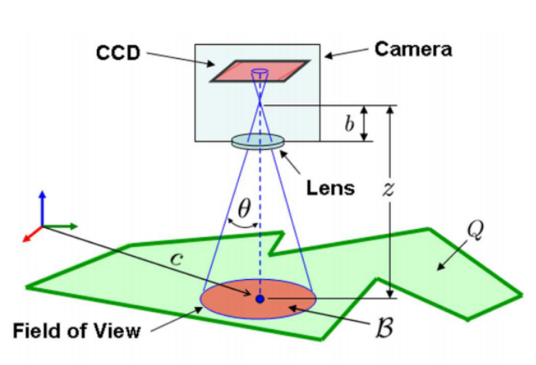
\includegraphics[width=2.5in]{MIT_pic}
\caption{Diagram of Major Parameters (from MIT Paper)}
\label{major_params}
\end{figure}

%%%%%%%%%%%%%%%%%%%%%%%%%%%
%Minimizing the Number of Altitude Changes and the Number of Turns
%%%%%%%%%%%%%%%%%%%%%%%%%%%

\section{Minimizing the Number of Turns and Number of Altitude Changes}
The proposed algorithm to minimize both the number of turns and altitude changes is based on Huang's MSA algorithm \cite{huang2001optimal}. Essentially, $Q$ is discretized into a set of disjoint polygons by clustering regions of similar $\psi(q)$ values together. Within each polygon, the UAV will fly under a constant altitude and can change its focal length if need be. In each polygon, the range in $\psi(q)$ values corresponds to no more than a $p$\% change in footprint size. This algorithm can be seen in Algorithm \ref{alg:MSA}.

The reasons why we chose this algorithm are multifold. First, by discretizing the regions into clusters of similar $\psi(q)$ values, we can lower the number of altitude changes. Secondly, the $p$\% threshold in footprint size difference helps minimize the number of turns as it allows the UAV to travel linearly in a boustrophedon format within each polygon. If $p$ were too big, then the footprint size would vary too much, and thus the traversal path of the UAV cannot be modelled by straight parallel lines. Instead, the UAV would have to turn more often to fully cover a given area. Discretizing the regions also helps to prevent the UAV from flying with an unnecessarily small footprint size in regions that have low $\psi(q)$ values, as small footprint sizes translates into the need for more parallel lines, and thus a larger number of turns.

\begin{algorithm}
\begin{algorithmic}[1]
\STATE $K$ = ClusteringAlgorithm() \COMMENT{Refer to Section \ref{clustering}}
\FOR{$k \in K$}
\STATE MSA($k$) \COMMENT{MSA($k$) fills polygon $k$ with parallel lines oriented to minimize the number of these lines.}
\ENDFOR
\end{algorithmic}
\caption{MSA Algorithm} 
\label{alg:MSA}
\end{algorithm}

%%%%%%%%%%%%%%%%%%%%%%%%%%%
%Clustering Algorithms
%%%%%%%%%%%%%%%%%%%%%%%%%%%

\section{Discretizing $Q$ via a Clustering Algorithm} \label{clustering}
While there are numerous heuristic clustering algorithms that exist in literature \cite{xu2005survey}, it is evident that for our problem, a clustering algorithm that both minimizes the number of clusters and intra-cluster $\psi(q)$ variance must be used in order to minimize the number of altitude changes and rotations. Because of the difficulty in knowing how small the variance should be within each cluster, a defined constant percentage threshold $p$ in footprint size can be used. As mentioned before, minimizing the footprint size in each polygon is paramount, as it allows the UAV to travel in straight lines, thereby reducing the number of rotations.

Our objective for the clustering algorithm can be defined as follows.

Given $G=(V,E)$ as an unweighted connected graph, where the vertices $V$ are all $\psi(q)$ values in $Q$, and $E$ is the set of edges that represent the adjacency of the $\psi(q)$ values in $Q$, minimize $K$ where $V_1, V_2, ..., V_K$ are connected and disjoint subsets of $V$. In addition, if we define $B_i$ as the set of footprint sizes corresponding to each $\psi(q)$ value in $V_i$, $\frac{B_{i_{max}}-B_{i_{min}}}{B_{i_{min}}} \leq p$ for $i = 1...K$.

%%%%%%%%%%%%%%%%%%%%%%%%%%%%%%%
%Agglomerative Hierarchical Clustering via Ward's Method
%%%%%%%%%%%%%%%%%%%%%%%%%%%%%%%
\subsection{Hierarchical Clustering via Ward's Method}
Because there are such a large number of clustering algorithms, only two were chosen in the scope of this research. Of course, further research should be done in determining the best clustering algorithm.

One of the two clustering algorithms chosen is the well-known agglomerative hierarchical clustering algorithm. Agglomerative hierarchical clustering is where individual $\Uppsi(q)$ values are initialized as clusters of their own, and with each iteration of the algorithm, smaller clusters form into larger clusters, until a stopping point is reached. While there are several methods in choosing the pair of clusters to merge at each iteration, Ward's method was chosen for our problem, as it fits our objective of minimizing intra-cluster variance of both $\psi$ and of footprint size \cite{ward1963hierarchical}. Only the two clusters with the minimum increase in sum-of-squared errors will be merged at each iteration. To put it more formally, a merge of two clusters $C_i$ and $C_j$ only occurs when the pair, $C_i$ and $C_j$, specifically results in the lowest value of the following objective function out of all cluster-pair combinations:
\begin{multline} \label{eq:ward_formula}
\Delta(C_i,C_j) = \sum_{k \in C_i \cup C_j} ( \psi_k - \mu_{C_i \cup C_j} )^2 \\
 - \Big( \sum_{k \in C_i} ( \psi_k - \mu_{C_i} )^2 + \sum_{k \in C_j} ( \psi_k - \mu_{C_j} )^2 \Big)
\end{multline}
\begin{equation}
\Delta(C_i,C_j) = \frac{n_{C_i}n_{C_j}}{n_{C_i} + n_{C_j}} (\mu_{C_i} - \mu_{C_j})^2
\end{equation}
Where $\mu_{C_i}$ corresponds to the average $\Uppsi$ value in cluster $C_i$.

Agglomerative hierarchical clustering algorithms need a defined stopping point or else the algorithm will continue until all clusters are merged into one. For our application, we can determine this stopping point by using the user-defined $p$ value. As soon as a merged cluster crosses the $p$ variance threshold, the algorithm ceases.

The clustering algorithm via Ward's method for our specific application is shown in Algorithm \ref{alg:clustering_3}. Note that $M$ is a symmetric matrix that stores and keeps track of $\Delta(C_i,C_j)$ for every cluster-pair combination. Also note that if two clusters are not adjacent to each other, then $\Delta(C_i,C_j) = \infty$. The time complexity for Algorithm \ref{alg:clustering_3} is $O(n^2)$.

%%TODO: ttps://en.wikipedia.org/wiki/Ward's_method (a faster way of doing HAC)
\begin{algorithm}
\begin{algorithmic}[1]
\STATE Initialize each $\psi(q) \in \Uppsi(q)$ as its own cluster $c \in C$.
\STATE Initialize graph $G$. \COMMENT{G holds every $\Uppsi(q)$ value and its adjacent relationships to other $\Uppsi(q)$ values.}
\STATE Initialize $p$. \COMMENT{$p$ is the percentage footprint size threshold.}
\STATE Initialize $currMaxVar \leftarrow 0$.
\WHILE{$C.size > 1$}
\STATE Initialize $minDelta \leftarrow \infty$.
\STATE Initialize $cluster_1 \leftarrow \emptyset$ and $cluster_2 \leftarrow \emptyset$.
\FOR{$i = 1$ to $G.Edges.Size$}
\STATE $M \leftarrow \Delta(G.Edges[i].cluster1, G.Edges[i].cluster2)$ \COMMENT{refer to Equation \ref{eq:ward_formula} for delta.}
\IF{$M \leq minDelta$}
\STATE $minDelta \leftarrow M(i, j)$
\STATE $cluster_1 \leftarrow G.Edges[i].cluster1$
\STATE $cluster_2 \leftarrow G.Edges[i].cluster2$
\ENDIF
\ENDFOR
\STATE $b_{min} \leftarrow getMinFP( cluster_1, cluster_2 )$
\STATE $b_{max} \leftarrow getMaxFP( cluster_1, cluster_2 )$
\IF{$\frac{b_{max}-b_{min}}{b_{min}} \geq p$}
\RETURN \COMMENT{Done merging clusters.}
\ELSE
\STATE mergeClusters($cluster_1$, $cluster_2$)
\ENDIF
\ENDWHILE
\end{algorithmic}
\caption{ClusteringAlgorithm()} 
\label{alg:clustering_3}
\end{algorithm}

%%%%%%%%%%%%%%%%%%%%%%%%%%%%%%%
%Lower Bound for Clustering Algorithm
%%%%%%%%%%%%%%%%%%%%%%%%%%%%%%%
\subsection{Clustering Algorithm Lower Bound}

It is evident that we cannot find a guarantee to this clustering algorithm without making heavy assumptions on the connectivity of the $\Uppsi$ graph in $Q$. Therefore, we attempt to output a lower bound for $K$ by relaxing the connectivity constraint, and only cluster similar $\Uppsi$ values together, regardless of whether or not two similar $\Uppsi$ values are necessarily adjacent in $Q$. To do this, $J$ and all $\psi$ points in Q, $\Uppsi$, must be given. This lower bound essentially is the specific scenario when all $\Uppsi$ values that are very similar to each other are all coincidentally adjacent to each other. There is no guarantee that our algorithm will give a value of $K$ close to this lower bound. However, outputting this lower bound and comparing it with the outputted $K$ from our algorithm can be of use, and with experimental evidence, we can see if our clustering algorithm can be within a small constant factor from the lower bound.

This type lower bound on $K$ can be found by Algorithm \ref{alg:lowerboundclustering}. Essentially, this algorithm goes through the sorted list of $\Uppsi$ from beginning to end and greedily clusters the $\Uppsi$ values. Note that the $\Uppsi$-range of every cluster is the same and must be equal to $J$.

\begin{algorithm}
\begin{algorithmic}[1]
\STATE $tempPsi \leftarrow \Uppsi[1]$
\STATE $lowerBoundK \leftarrow 1$
\FOR{$\psi \in \Uppsi$}
\IF{$\psi > tempPsi + p$}
\STATE $tempPsi \leftarrow \psi$
\STATE $lowerBoundK \leftarrow lowerBoundK + 1$
\ENDIF
\ENDFOR
\RETURN $lowerBoundK$
\end{algorithmic}
\caption{LowerBound($J$, $\Uppsi$)} 
\label{alg:lowerboundclustering}
\end{algorithm}

\subsubsection{Proof of Correctness for Lower Bound}
The logic that we use is very similar to the proof of correctness we use for our greedy focal length controller.

To prove the optimality of our algorithm, we must first prove that our algorithm exhibits both the greedy choice property and the optimal substructure property.
\begin{lemma} %greedy choice property
Let us define the first step of our algorithm, $d_1$. $d_1$ finds the first interval, $[\psi_1, \psi_i]$, that represents the first cluster we greedily find based off of the first $\Uppsi$ value in the sorted $\Uppsi$ list, $\psi_1$. Then, there always exists an optimal solution $S^*$ in which $d_1$ is its first step.
\end{lemma}
The following proves this greedy choice property. Let $R$ be defined as one optimal solution. If $R$ already includes $d_1$, then the property holds and is trivial. If $R$ does not include $d_1$, then there is only one possibility: the first step in $R$ starts at a value of $\Uppsi$ less than $\psi_1$. The first cluster cannot start at a $\Uppsi$ value greater than $\psi_1$ or else $\psi_1$ will not be in any cluster at all. Let us call this first step of $R$ as $d_{R_1}$.

We can exchange $d_{R_1}$ that was originally from $R$ with our first step, $d_1$, very easily, even if the second cluster in $R$, $d_{R_2}$, is directly adjacent to $d_{R_1}$. We can simply remove $d_{R_1}$, shorten $d_{R_2}$ such that its interval starts right after $\psi_i$, where $\psi_i$ is the value $d_1$ ends, and then finally place $d_1$ into R. Thus, the following holds true: $d_{R_1}$ can be exchanged with $d_1$ in $R$, to produce another solution, $S^*$, which is still optimal.

\begin{lemma} %optimal substructure property
Let $S'$ denote the sequence of a minimum number of disjoint clusters, where the total range of all the clusters is between $(\psi_i, \psi_n]$, where $\psi_i$ is the last point in the first cluster (whatever the first cluster may be), and where $\psi_n$ is the last $\Uppsi$ value in the sorted list. Then, $S = \langle d_1, S' \rangle$ must be an optimal solution.
\end{lemma}
We now prove this optimal substructure property. We know that none of the clusters in sequence $S'$ overlap with $d_1$. Thus, $S = \langle d_1, S' \rangle$ is a feasible solution. We also know from the last lemma, there exists an optimal sequence $S^*$ in which $d_1$ is its first cluster. It is apparent that $S^* - d_1$ is also compatible with $d_1$. Since $S'$ was defined to be an optimal sequence for $[q_i, q_n]$, then the following inequality holds:
\begin{equation*}
\lvert S' \rvert \leq \lvert S^* - d_1 \rvert \\
\end{equation*}
Thus, we can apply the following logic:
\begin{gather*}
\lvert S^* - d_1 \rvert = \lvert S^* \rvert -1 \\
\lvert S' \rvert \leq \lvert S^* \rvert -1 \\
\lvert S \rvert = \lvert S' \rvert + 1 \\
\lvert S \rvert -1 = \lvert S' \rvert \\
\lvert S \rvert -1 \leq \lvert S^* \rvert -1 \\
\lvert S \rvert \leq \lvert S^* \rvert 
\end{gather*}
Thus, S is an optimal solution.

Finally, we can prove the correctness of this algorithm by induction:
\begin{enumerate}
\item Basis: If $\lvert S \rvert = 1$, the algorithm gives us an optimal solution, as $d_1$ is already optimal.
\item Induction Step: Assume our algorithm can give us optimal solutions for all sequences where the number of clusters is $z$, for some $z \geq 1$. We show that our algorithm also provides an optimal solution for sequences of clusters of size $z+1$. Consider a coverage path where the optimal solution results in $z+1$ intervals. By the greedy choice property, $d_1$, obtained from our algorithm, is part of some optimal solution for this problem. By the optimal substructure property, after $d_1$, there is an $S'$ that can be combined with $d_1$ to give us an optimal solution, $S=\langle d_1, S' \rangle$. $S'$ has to consist of $z$ steps. We already assumed we can solve problems of size $z$, and thus, using the logic above, we can also solve $S$, or more generally, problems of size $z+1$.
\end{enumerate}


\subsection{User-Defined Polygonal Decomposition of $\Uppsi(q)$} 
Instead of the above two methods, we could disregard the concept $\Uppsi(q)$ entirely and instead use a completely different way to describe the minimum required resolution over sub-regions in area $Q$. We could instead have the end-user manually tell us convex polygons over $Q$ in which there is a uniform minimum resolution required. For example, using a Google Maps-like application, the user can draw polygons over sub-regions of $Q$ where there needs to be better or worse resolution than the rest of $Q$. If the user requests a concave polygon shape to have a certain $\Uppsi(q)$ value, we can break the concave polygon into multiple convex polygons in order to get a smaller amount of lines, and thus a smaller number of rotations, than if we were to keep the concave polygon intact\textemdash similar to Bochkarev and Smith \cite{bochkarevminimizing}.

%%%%%%%%%%%%%%%%%%%%%%%%%%%
%CGTSP Tour Generation
%%%%%%%%%%%%%%%%%%%%%%%%%%%
\section{Clustered GTSP (CGTSP) Tour Generation}

In Bochkarev and Smith \cite{bochkarevminimizing}, a GTSP (generalized travelling salesman problem) solver was used in order to plan a coverage path of disjoint polygons, where within each polygon, straight parallel lines oriented along the polygon's longest height are traversed. For graph $G=(V,E)$ where $V=\{v_i...v_n\}$ is the set of all vertices and $E=\{(v_i,v_j) ; v_i, v_j \in V, i \neq j\}$ is the set of all edges, the GTSP is defined such that the set $V$ is further subdivided into subsets $V_1...V_k$, where $k$ is the number of subsets, $V_1\cup V_2 \cup ... V_k = V$, and that for all subsets $V_i$ and $V_j$, where $i \neq j$, $V_i \cap V_j = \emptyset$. Solving the GTSP requires finding the shortest path such that we visit only one node for every subset. For both Bochkarev and Smith's problem and our problem, each straight line can be traversed in two possible ways. Thus, every vertex should represent one way of traversal for one line, and every subset has a size of 2, and represents the two possible traversal paths of a line.

In contrast to the GTSP, a clustered TSP (CTSP) solver is a bit different. In a CTSP, every time the traveler goes into a cluster, they must travel to every node within the same cluster before moving onto another cluster. 

A CGTSP is a combination of the two above problems, and must be solved in our specific problem. To clarify, a CGTSP is where the subsets from a GTSP are clustered such that the travelling salesman needs to travel to every subset within the same cluster of subsets before going onto the next cluster of subsets.

Therefore, our graph $G = (V, E)$ is defined such that each $v_i \in V$ represents a line that the UAV traverses in one of two possible directions. Similar to Bochkarev and Smith's GTSP, each subset in our problem consists of only two nodes, representing the two possible traversal directions. The weight of each edge in $E$ represents the cost of travel for the UAV from one line to another. In our simulations, we utilize Dubins' car model to calculate these edge weights. Every cluster of subsets in this CGTSP represents a polygon obtained from the clustering algorithm mentioned in Section \ref{clustering}. These clusters of polygons of similar altitudes need to be consecutively travelled one at a time in order to minimize the number of altitude changes, which is why we could not use the simple GTSP solver from Bochkarev and Smith.

\subsection{Reduction of CGTSP into GTSP}

No solver for CGTSP exists in literature as of yet. However, the previous two types of problems, GTSP and CTSP, have been solved by reducing the problems to a simple ATSP \cite{helsgaun2015solving} and TSP problem \cite{helsgaun2011solving}, respectively. The CGTSP solver can be solved in a similar way to these two, by reducing it into a GTSP. The transformation, similar to that of Helsgaun's \cite{helsgaun2011solving}, is described below where $V'$ is the transformed vertex set, $V_i'$ is the $i$th transformed subset of vertices, and $c'_{ij}$ represents the new transformed cost between vertices $v_i$ and $v_j$:

\begin{enumerate}[label=(\alph*)]
\item $V = V'$
\item $\{V_1...V_k\} = \{V_1'...V_k'\}$
\item Define $c_{ij}' = c_{ij}$, when $v_i$ and $v_j$ belong to the same cluster.
\item Define $c_{ij}' = c_{ij} + M$, when $v_i$ and $v_j$ belong to two different clusters. $M$ is a large constant, where $\sum_{(i,j) \in V} c_{ij} < M < \infty$ \cite{noon1993efficient}.
\end{enumerate}

When entering a cluster at a vertex $v_i$, an optimal GTSP tour will always visit all other vertex sets of the cluster before moving to the next cluster due to the added $M$ term for inter-cluster edges. If we define $m$ as the number of inter-cluster edges the GTSP tour will have, then cost of the tour for the actual CGTSP is the cost of the above CGTSP-to-GTSP tour subtract $mM$.

%%%%%%%%%%%%%%%%%%%%%%%%%%%
%Focal Length Controller
%%%%%%%%%%%%%%%%%%%%%%%%%%%

\section{Focal Length Controller}

We have made several assumptions for the focal length controller. First, the camera uses parfocal lens rather than varifocal lens. Varifocal lens are used by most standard cameras, where they take a set amount of time to be refocused. Parfocal lens, on the other hand, stays in focus even when the focal length is changed. Thus, parfocal lens is more practical in aerial surveillance for a fixed-wing UAV since there will not be any waiting duration for the camera to refocus while the aircraft is flying over the coverage area.
The second assumption we made is that the UAV can accurately estimate its altitude over Q. There are various papers that cover altitude estimation for UAVs, including \cite{eynard2010uav} and \cite{cherian2009autonomous}.
Thirdly, we do not consider digital zoom at all. This section entirely deals with optical zoom. Digital zoom is undesirable as it is analogous to merely cropping the original image and enlarging it, which severely affects resolution.

In addition to these assumptions, an equation relating $\psi$ with the altitude of the UAV, $z$, and the UAV's focal length, $f$, must be derived.

Given that $n$ is the total number of pixels for the camera and $b$ is the footprint size:
% Defining psi
\begin{equation}
\psi =  \frac{n}{\pi b^2}
\end{equation}
We can also define $b$ in terms of the UAV's altitude, $z$, the size of the sensor, $s$, and the focal length, $f$ by understanding that the relationship between them comes from similar triangles:
% Defining B as a circular area
\begin{equation}
b = z \frac{s}{2f}
\end{equation}
Note that half the length of the sensor is used, $\frac{s}{2}$, due to the fact that $b$ is only the radius of the footprint and not the diameter.
Combining the two above equations together results in the following relationship:
% The complete equation used in the focal length controller
\begin{equation} \label{eq:psi_z_f}
\psi = \frac{n}{\pi \left(\frac{zs}{2f}\right)^2}
\end{equation}

%Greedy Focal Length Controller
\subsection{Greedy Focal Length Controller}
An offline greedy focal length controller was devised using Equation \ref{eq:psi_z_f} and by minimizing the following cost function in order to minimize the number of altitude changes.

Let us define a function $f(x)$ where $x \in [0, x_n]$. Let us also define a set $f_1, f_2, ... f_n$ where:
\begin{align}
& f_1(x) = f(x) : x \in [0, x_1]\\
& f_2(x) = f(x) : x \in (x_1, x_2]\\
& ... \\
& f_n(x) = f(x) : x \in (x_{n-1}, x_n]
\end{align}
so that:
\begin{equation*}
 f(x)=  \left\{
\begin{array}{ll}
      f_1(x) & \text{for } [0,x_1] \\
      f_2(x) & \text{for } (x_1,x_2] \\
      ...\\
      f_n(x) & \text{for } (x_{n-1},x_n] \\
\end{array} 
\right.
\end{equation*}
Also define $g_i = max(f_i(x))$ and $h_i = min(f_i(x))$.
Our objective function is to minimize $n$:
\begin{gather} \label{eq:focal_cost}
C_{focal} = n
\tag*{\text{such that } $g_i/h_i \leq F$ \text{for } $i = 1...n$}
\end{gather}
Where $C_{focal}$ is the cost function, $F$ is a constant, and wherever the condition $g_i/h_i \leq F$ breaks is where $f_{i+1}$ starts. 

In our specific application, $f(x)$ is $\Uppsi(q)$, and $F$ is the range of possible resolutions that can be achieved by solely changing the focal length of the camera, without the altitude. This range can be derived from the following:
\begin{equation}
g_i = \frac{n}{\pi \left( \frac{z_i s}{ 2 f_{max}} \right)^2}
\end{equation}
\begin{equation}
h_i = \frac{n}{\pi \left( \frac{z_i s}{ 2 f_{min}} \right)^2}
\end{equation}
\begin{equation}
\frac{ g_i }{ h_i } = \left( \frac{ f_{max} }{ f_{min} } \right)^2
\end{equation}
\begin{equation} \label{eq:maxresolutionrange}
F = \left( \frac{ f_{max} }{ f_{min} } \right)^2
\end{equation}

With the above equation, we can figure out where along the traversal path the intervals should be. The next step is to figure out what altitude the UAV should fly at for each interval. The following derives the correct altitude value, $z_i$, for $(x_i,x_{i+1}]$:
\begin{equation} \label{eq:altitude_from_g}
z_i = \frac{2f_{max}}{s} \sqrt{\frac{n}{\pi g_i}}
\end{equation} 
\begin{equation} \label{eq:altitude_from_h}
z_i = \frac{2f_{min}}{s} \sqrt{\frac{n}{\pi h_i}}
\end{equation}
By adding Equations \ref{eq:altitude_from_g} and \ref{eq:altitude_from_h} together and re-arranging, we get $z_i$:
\begin{equation} \label{eq:z_for_interval}
z_i = \frac{ \sqrt{\frac{n}{\pi}} \left( \frac{f_{max}}{\sqrt{g}} + \frac{f_{min}}{\sqrt{h}} \right) }{s}
\end{equation}

Algorithm \ref{alg:focal_global_alt} uses Equations \ref{eq:maxresolutionrange} and \ref{eq:z_for_interval} to find the optimal altitudes for the UAV change throughout the coverage path in order to minimize the cost function. Note that this algorithm assumes we already have a known traversal path to cover area $Q$ from the CGTSP. Also note that this algorithm is run strictly before the UAV actually travels along the coverage path. The algorithm returns the tuple-list object, $P$, which is used to figure out at what points along the coverage path from $q_i$ to $q_m$, called $CP$, the altitude must change, and also the exact value the altitude of the UAV must be changed to. Algorithm \ref{alg:focal_global} is run while the UAV is operating. This algorithm uses the tuple list obtained from Algorithm \ref{alg:focal_global_alt} in order to change the altitude of the UAV as the UAV travels along the coverage path. 

Finally, the time complexity of both algorithms \ref{alg:focal_global_alt} and \ref{alg:focal_global} is $O(n)$, where $n$ in this case is the number of discrete steps in the coverage path $CP$.

%Greedy Function to Determine When Altitude must be Changed for Greedy Focal Length Controller
\begin{algorithm}
\begin{algorithmic}[1]

\STATE $P \leftarrow \emptyset$ \COMMENT{where $P$ is a list of tuples. Each tuple has one position value of $q \in Q$, and one altitude value $z$.}
\STATE $g \leftarrow \Uppsi(q_1)$ \COMMENT{where $q_1$ is the first area the UAV will be while traversing along the coverage path.}
\STATE $h \leftarrow \Uppsi(q_1)$
\FOR[where m is the number of ordered elements in $Q$ that make up the traversal path of the UAV, $CP$]{$i = 2 \text{ to } m$}
\IF{$\Uppsi(q_i) > g$}
\STATE $g \leftarrow \Uppsi(q_i)$
\ENDIF

\IF{$\Uppsi(q_i) < h$}
\STATE $h \leftarrow \Uppsi(q_i)$
\ENDIF

\IF{$ \frac{g}{h} \geq \left( \frac{ f_{max} }{ f_{min} } \right)^2 $}
\STATE $z_i = \frac{ \sqrt{\frac{n}{\pi}} \left( \frac{f_{max}}{\sqrt{g}} + \frac{f_{min}}{\sqrt{h}} \right) }{s}$ \COMMENT{from Equation \ref{eq:z_for_interval}}
\STATE $p \leftarrow (q_i, z_i)$
\STATE $P.append(p)$
\STATE $g \leftarrow \Uppsi(q_i)$
\STATE $h \leftarrow \Uppsi(q_i)$
\ENDIF

\ENDFOR
\RETURN P
\end{algorithmic}
\caption{Offline Greedy Function to Determine When Altitude Must be Changed}
\label{alg:focal_global_alt}
\end{algorithm}

%Greedy Focal Length Controller Algorithm
\begin{algorithm}
\begin{algorithmic}[1]

\STATE Let $f$ be the current focal length, and $z$ be the current altitude. Let $P$ be the list of tuples obtained from Algorithm \ref{alg:focal_global_alt}.
\FOR{$i = 1 \text{ to } m$}
\IF{$q_i = P[0].q$}
\STATE $z \leftarrow P[0].z$
\STATE Pop $P[0]$ from $P$.
\ENDIF
\STATE $f \leftarrow \frac{zs}{2} \sqrt{\frac{\pi\psi}{n}}$
\ENDFOR

\end{algorithmic}
\caption{Greedy Focal Length Controller}
\label{alg:focal_global}
\end{algorithm}

%Proof of Correctness
\subsubsection{Proof of Correctness}
This section establishes the correctness of Algorithms \ref{alg:focal_global_alt} and \ref{alg:focal_global} and proves why this greedy controller produces an optimal number of altitude changes for a given coverage path.

To prove the optimality of our algorithm, we must first prove that our algorithm exhibits both the greedy choice property and the optimal substructure property.
\begin{lemma} %greedy choice property
Let us define the first step of our algorithm, $d_1$. $d_1$ finds the first interval, $[q_0, q_i]$, that greedily maximizes the distance travelled until the UAV must change altitude. Then, there always exists an optimal solution $S^*$ in which $d_1$ is its first step.
\end{lemma}
The following proves this greedy choice property. Let $R$ be defined as one optimal solution. If $R$ already includes $d_1$, then the property holds and is trivial. If $R$ does not include $d_1$, and instead has its first step as $d_{R_1}$ with an interval $[q_{R_0}, q_{R_i}]$, where $d_{R_1} \neq d$, then $q_{R_i} < q_i$, since $d_1$ was already defined as the maximum interval possible before the maximum camera resolution range condition breaks. From this, we can exchange the original interval $[q_{R_0}, q_{R_i}]$ in $R$ with $[q_0, q_i]$. Note that in order to do so, the interval of difference between $d_1$ and $d_{R_1}$, $[q_{R_i}, q_i]$, that was originally in the second step interval in $R$, $d_{R_2}$, will move into the first step interval. This transferal process is valid as it does not violate the maximum camera resolution range condition for the second step interval, $d_{R_2}$. Thus, the following holds true: $d_{R_1}$ can be exchanged with $d_1$ in $R$, to produce another solution, $S^*$, which is still optimal. The only difference now between $R$ and $S^*$ is that the altitude value at which the UAV must fly in the first interval will change, though this does not affect the proof in any way.
\begin{lemma} %optimal substructure property
Let $S'$ denote an optimal sequence of intervals between $(q_i, q_n]$, where $q_i$ is the last point in the first interval (whatever the first interval may be), and $q_n$ is the last point in the coverage path. Then, $S = \langle d_1, S' \rangle$ must be an optimal solution.
\end{lemma}
We now prove this optimal substructure property. We know that none of the intervals in sequence $S'$ overlap with $d_1$. Thus, $S = \langle d_1, S' \rangle$ is a feasible solution. We also know from the last lemma, there exists an optimal sequence $S^*$ in which $d_1$ is its first interval step. It is apparent that $S^* - d_1$ is also compatible with $d_1$. Since $S'$ was defined to be an optimal sequence for $[q_i, q_n]$, then the following inequality holds:
\begin{equation*}
\lvert S' \rvert \leq \lvert S^* - d_1 \rvert \\
\end{equation*}
Thus, we can apply the following logic:
\begin{gather*}
\lvert S^* - d_1 \rvert = \lvert S^* \rvert -1 \\
\lvert S' \rvert \leq \lvert S^* \rvert -1 \\
\lvert S \rvert = \lvert S' \rvert + 1 \\
\lvert S \rvert -1 = \lvert S' \rvert \\
\lvert S \rvert -1 \leq \lvert S^* \rvert -1 \\
\lvert S \rvert \leq \lvert S^* \rvert 
\end{gather*}
Thus, S is an optimal solution.

Finally, we can prove the correctness of this algorithm by induction:
\begin{enumerate}
\item Basis: If $\lvert S \rvert = 1$, the algorithm gives us an optimal solution, as $d_1$ is already optimal.
\item Induction Step: Assume our algorithm can give us optimal solutions for all sequences where the number of intervals is $z$, for some $z \geq 1$. We show that our algorithm also provides an optimal solution for sequences of size $z+1$. Consider a coverage path where the optimal solution results in $z+1$ intervals. By the greedy choice property, $d_1$ is part of some optimal solution for this problem. By the optimal substructure property, after $d_1$, there is an $S'$ that can be combined with $d_1$ to give us an optimal solution, $S=\langle d_1, S' \rangle$. $S'$ has to consist of $z$ steps. We already assumed we can solve problems of size $z$, and thus, using the logic above, we can also solve $S$, or more generally, problems of size $z+1$.
\end{enumerate}

\subsubsection{Minimizing Total Distance in Change of Altitude}
Not only does this algorithm minimize the number of altitude changes, but it also minimizes the total distance of change in altitude.
\begin{claim} %minimum total distance in altitude change
The greedy focal length controller algorithm minimizes the total distance in change of altitude for the UAV.
\end{claim}
We prove this via proof of contradiction. We know that our algorithm produces the minimum number of intervals for path $CP$ from the proof of correctness in the previous section, which directly corresponds to a minimum number of altitude shifts. Let this minimum number of altitude shifts be $w$. Thus, the only case we have to consider is the case in which there are more than $w$ altitude shifts.

Take some arbitrary interval from point $q_i$ to some point $q_j$, where $q_j > q_i$, such that our algorithm will have one altitude shift. Define this altitude shift's distance as $H$. Let us assume there exists another algorithm that gives this interval $[q_i, q_j]$ a larger number of altitude shifts, $n$, where $n \geq 2$, and where the total distance in altitude change is defined as $H_* = h_1 + h_2 + ... + h_n$. Additionally assume that $H_* < H$, which means $h_1 + h_2 + ... + h_n < H$. However, if this inequality holds true, then there must exist at least one $\Uppsi(q)$ point along the coverage path that cannot be reached purely changing the focal length of the camera, since we have shortened the total altitude distance to $H_*$. To compensate for this, we must add more altitude shifts. However, by then, $h_1 + h_2 + ... + h_n + h_{n+1} + ... \geq H$. Thus, by proof of contradiction, there is no such total altitude distance $H_*$, where $H_* < H$, that can fully cover the desired minimum-required resolutions without changing altitude at another $q$ point between $[q_i, q_j]$. This reasoning can be extended to the entire coverage path, $CP$, where the following inequality must be true: $H(w+n) \geq H$, where $H(w+n)$ is the total altitude distance when there are $w+n$ number of altitude shifts, and where $n \geq 1, n \in \mathds{Z}$. Therefore, our algorithm does indeed minimize the total distance in change of altitude.

To summarize, once you decrease the value of $H$ from our algorithm to a smaller value, there will exist $\Uppsi(q)$ points that cannot be reached without creating additional altitude shifts to compensate. The total $H_*$, including the additional altitude shifts, will be at least equal to our original $H$. Thus, our $H$ must be the minimum.

\section{Simulations}
The simulation results goes here.

\section{Conclusion}
The conclusion goes here.


% trigger a \newpage just before the given reference
% number - used to balance the columns on the last page
% adjust value as needed - may need to be readjusted if
% the document is modified later
%\IEEEtriggeratref{8}
% The "triggered" command can be changed if desired:
%\IEEEtriggercmd{\enlargethispage{-5in}}

% references section

% can use a bibliography generated by BibTeX as a .bbl file
% BibTeX documentation can be easily obtained at:
% http://mirror.ctan.org/biblio/bibtex/contrib/doc/
% The IEEEtran BibTeX style support page is at:
% http://www.michaelshell.org/tex/ieeetran/bibtex/
\bibliographystyle{IEEEtran}
% argument is your BibTeX string definitions and bibliography database(s)
\bibliography{bib/ref}

% <OR> manually copy in the resultant .bbl file
% set second argument of \begin to the number of references
% (used to reserve space for the reference number labels box)
%\begin{thebibliography}{1}
%\bibitem{IEEEhowto:kopka}
%H.~Kopka and P.~W. Daly, \emph{A Guide to \LaTeX}, 3rd~ed.\hskip 1em plus
% 0.5em minus 0.4em\relax Harlow, England: Addison-Wesley, 1999.
%\end{thebibliography}

% that's all folks
\end{document}


